\documentclass[12pt]{article}
\usepackage[utf8]{inputenc}
\usepackage[T1]{fontenc}
\usepackage[top=5em,bottom=10em]{geometry}


% LIST OF FIGURES AND TABLES 
\usepackage{tocloft}

\renewcommand{\cftfigpresnum}{Abb. }
\renewcommand{\cfttabpresnum}{Tab. }

\renewcommand{\cftfigaftersnum}{:}
\renewcommand{\cfttabaftersnum}{:}

\setlength{\cftfignumwidth}{2cm}
\setlength{\cfttabnumwidth}{2cm}

\setlength{\cftfigindent}{0cm}
\setlength{\cfttabindent}{0cm}


%just until it's fixed by MiKTeX###############
\makeatletter
\def\set@curr@file#1{%
  \begingroup
    \escapechar\m@ne
    \xdef\@curr@file{\expandafter\string\csname #1\endcsname}%
  \endgroup
}
\def\quote@name#1{"\quote@@name#1\@gobble""}
\def\quote@@name#1"{#1\quote@@name}
\def\unquote@name#1{\quote@@name#1\@gobble"}
\makeatother
%################################

\usepackage{graphicx}
\graphicspath{ {./images/} }
\usepackage{hyperref}
\geometry{a4paper}

\usepackage[ngerman]{babel}

\begin{document}

\title{Exposé\\\huge Desktopanwendung zur unterstützten Gestaltung von Origami Diagrammen\\\large Praxisprojekt WS 2019/2020}
\author{Julian Hardtung}
\date{\today}
\maketitle
%\tableofcontents
\renewcommand{\figurename}{Abb.}
\renewcommand{\tablename}{Tab.}
\section{Problemfeld \& Kontext}

Um Anleitungen für Origami-Figuren weltweit teilen und verbreiten zu können, wurden bestimmte Konventionen und Symbole zur Repräsentation von spezifischen Faltschritten bestimmt \cite{diagramming_conventions}. Um diese sogenannten Diagramme zu erstellen, wird jeder einzelne Schritt der Faltsequenz per Hand/virtuell (mit z.B. Adobe Illustrator oder Inkscape) gezeichnet, um den aktuellen Zustand des Papiers darzustellen. Dieser Prozess ist sehr zeitaufwändig und erfordert ein hohes Maß an Genauigkeit. Dies ist bei einfachen Modellen mit wenigen Schritten, wie dem klassischen Kranich, zunächst kein großes Problem %(siehe Abb. \ref{cranediagram}). 

\begin{figure}[h]
\centering
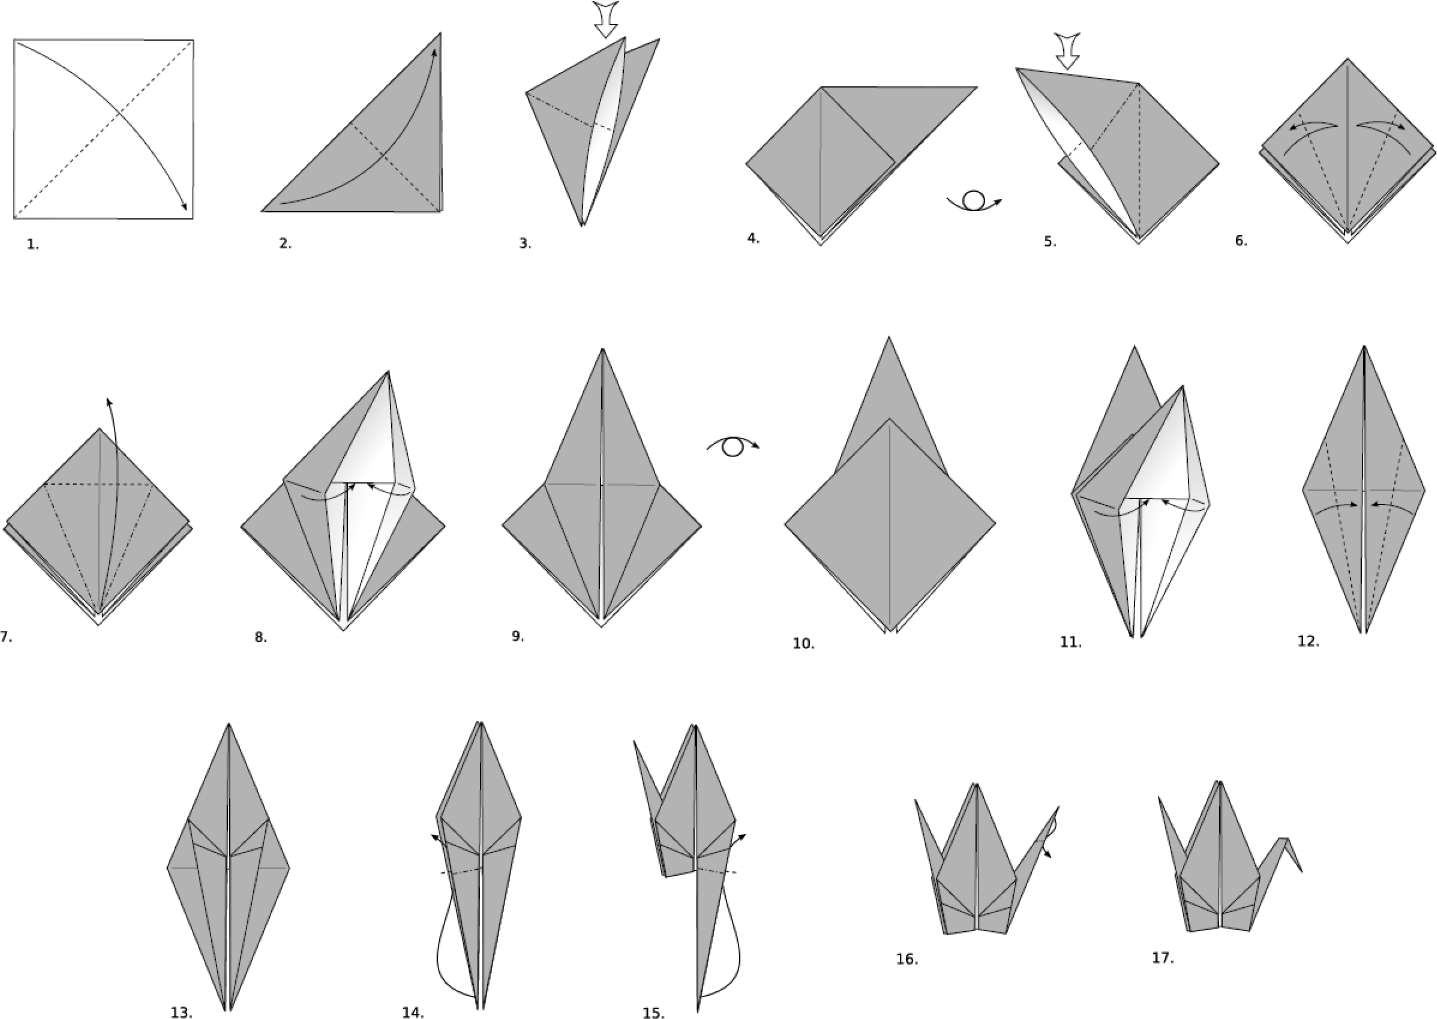
\includegraphics[width=0.75\textwidth]{crane1}
\caption{Origami Diagramm Kranich}
\label{fig:cranediagram}
\end{figure}

\newpage

Werden die Origami Modelle allerdings komplexer, so erhöht sich der Zeit-/ und Kostenaufwand für die Diagrammerstellung drastisch. Diagramme mit 200-300 einzelnen Schritten sind hier keine Seltenheit.

\begin{figure}[h]
\centering
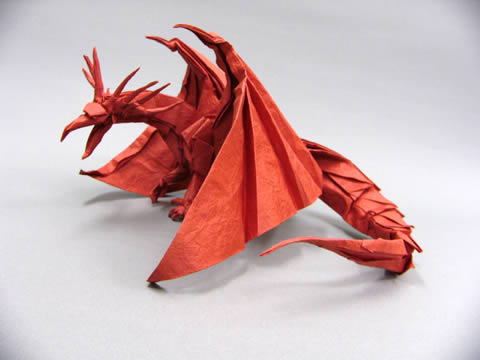
\includegraphics[scale=0.5]{ancientdragon.jpg}
\caption{Ancient Dragon von Satoshi Kamiya (274 Einzelschritte)}
\label{fig:ancientdragon}
\end{figure}


\section{Zielsetzung}
Ziel des Projektes ist es, eine Desktopanwendung zu entwickeln, welche den Benutzer bei der Erstellung von Origami Diagrammen unterstützt. Dafür muss zunächst ein Ist-Zustand definiert werden, in dem alle relevanten Symbole, Notationen und allgemeinen Regelungen gesammelt und kategorisiert werden. So können alle Elemente darauf untersucht werden, wie diese in dem zuvor erwähnten Tool implementiert werden können, um dem Benutzer die Arbeit zu erleichtern oder ganz abzunehmen.

Die Erweiterung auf ein vollkommen virtuelles Falten von Papier mit dreidimensionaler Ansicht wäre eine mögliche Überlegung für eine Bachelorarbeit.

\section{Ressourcen}\label{ressourcen}

Ein ähnliches Projekt wurde bereits von John Szinger mit  \textit{"The Foldinator Project"}\cite{foldinator} begonnen. Der Foldinator sollte das virtuelle Falten von Papier ermöglichen und so die einzelnen Schritte beim Falten eines Modelles aufnehmen und abspeichern. Dieses Projekt wurde allerdings seit 2009 nicht mehr aktualisiert und ist nie aus der frühen Prototypenphase herausgetreten.
Im Rahmen der Entwicklung des Foldinators schlug Szinger vor, Origami Diagramme in einem .xml-Format abzuspeichern\cite{origamixml}. Genauere Konventionen und Regelungen für das OrigamiXML wurden von Szinger genannt, allerdings vermutete er, dass einige Anpassungen vollzogen werden müssten:\\
 
\textit{``I fully expect there will be some back'n'forth between the XML and the engine to get the kinks ironed out.''}\footnote{John Szinger: Origami XML\cite{origamixml}}

Die 7 Huzita-Justin Axiome \cite{hj_axioms} beschreiben jede einzelne Origami Operation, die ausgeführt werden kann. Diese Axiome werden bei der späteren Implementation hilfreiche Anhaltspunkte bieten.

\section{Motivation}
Das Themengebiet um Origami bietet viele künstlerische Freiheiten und folgt dennoch strengen mathematischen Gesetzen (siehe Abschnitt \ref{ressourcen}: Huzita-Justin Axiome). Diese Aspekte interessieren mich schon seit langem und zeigen die Vielseitigkeit bei der Erstellung von Origami-Figuren. Die Motivation für das Praxisprojekt resultiert aus einem generellen Interesse am hobbymäßigen Falten von Origami-Figuren. In den letzten Jahren stellte sich immer mehr das Problem heraus, dass kaum neue, komplexe Diagramme herausgebracht werden. So wuchs die Motivation, den Prozess der Diagrammerstellung zu vereinfachen und zu optimieren.

\section{Chancen \& Risiken}
Bei späterer Nutzung des Tools insbesondere für komplexe Modelle könnten unvorhergesehene Probleme auftreten. Der Fokus soll allerdings zunächst auf Grundfunktionalität gesetzt werden, sodass alle Falttechniken und Symbole repräsentiert werden und nutzbar sind. Danach können eventuelle Probleme für komplexe Modelle in Angriff genommen werden und das Basisprogramm anhand dieser Probleme angepasst werden.

Weiterhin muss sichergestellt werden, dass die Anwendung bei späterer Nutzung eine tatsächliche Zeitersparnis gegenüber der bisher üblichen Methoden einbringt.

\section{Zeitplan}

05.11.2019 - 25.11.2019: 
\begin{itemize}
\item Recherche \& Planung
\item Anforderungsanalyse
\item Kategorisierung der etablierten Symbole und Konventionen
\item Technische Recherche (Architekturplanung)
\end{itemize}
26.11.2019 - 13.01.2020:
\begin{itemize}
\item Implementierung/ Umsetzung
\item Ausarbeitung mit Vorgehensweisen/Probleme/Erfolge
\end{itemize}


\newpage


\begin{thebibliography}{9}
\bibitem{diagramming_conventions}
Robert J. Lang: ORIGAMI DIAGRAMMING CONVENTIONS, 10.08.2011
\\\texttt{http://www.langorigami.com/article/origami-diagramming-conventions} [1.11.19]

\bibitem{foldinator}
John Szinger: The Foldinator Project,
\\\texttt{http://zingman.com/origami/foldinator.php} [1.11.19]

\bibitem{origamixml}
John Szinger: Origami Xml, Juli 2009
\\\texttt{http://zingman.com/origami/origamiXml.php} [1.11.19]

\bibitem{hj_axioms}
Robert J. Lang: HUZITA-JUSTIN AXIOMS, 23.09.2015
\\\texttt{https://langorigami.com/article/huzita-justin-axioms/} [1.11.19]
\end{thebibliography}


\listoffigures


\end{document}


